\section{Data and Methods}
\subsection{Pipelines data}
For this research, we use datasets provided by the US Federal Energy Regulatory Commission (FERC). The datasets merged together for this research encompass data on all American pipeline operators from the years 2004-2018. To ensure that datasets from different time periods are continuous, we plotted out the most important variables, and inspected the plot visually for discontinuities (Figure 1). We did not observe any discontinuity for the cutoff (2009/2010). FERC provides detailed data on e.g., energy production, transport, and consumption, that has been used in a variety of studies in the fields of management and econometrics. FERC's data on pipelines has only been used in one study so far, where the impact of incidents on reputation and networks is studied \citep{Park2019}. FERC provides, separately, data on both operators' scale of pipeline networks, and on incidents. Operators file separate for different commodities (e.g.,Crude Oil, Petroleum), and report accounts on details such as pipeline miles by decade, by welt type, by nominal pipe size, etc. Incidents are recorded with a similar level of detail: in the latest iteration of the report form encompasses 18 pages with several hundred items, including for instance time, longitude and latitude, the commodity transported, thickness, material and treatment of the pipe, the cause of the incident with several follow-up questions, details on the staff that worked on the section and so forth. Every year in our observation period, over 100 significant incidents have been reported, Figure 2 illustrates the scale of the phenomenon since 2010.

{\centering
	//////////////////////////////////////////////////////////////////////////////
	
	[Insert Figure 1 approximately here]
	
	//////////////////////////////////////////////////////////////////////////////\par
}

\begin{figure}
	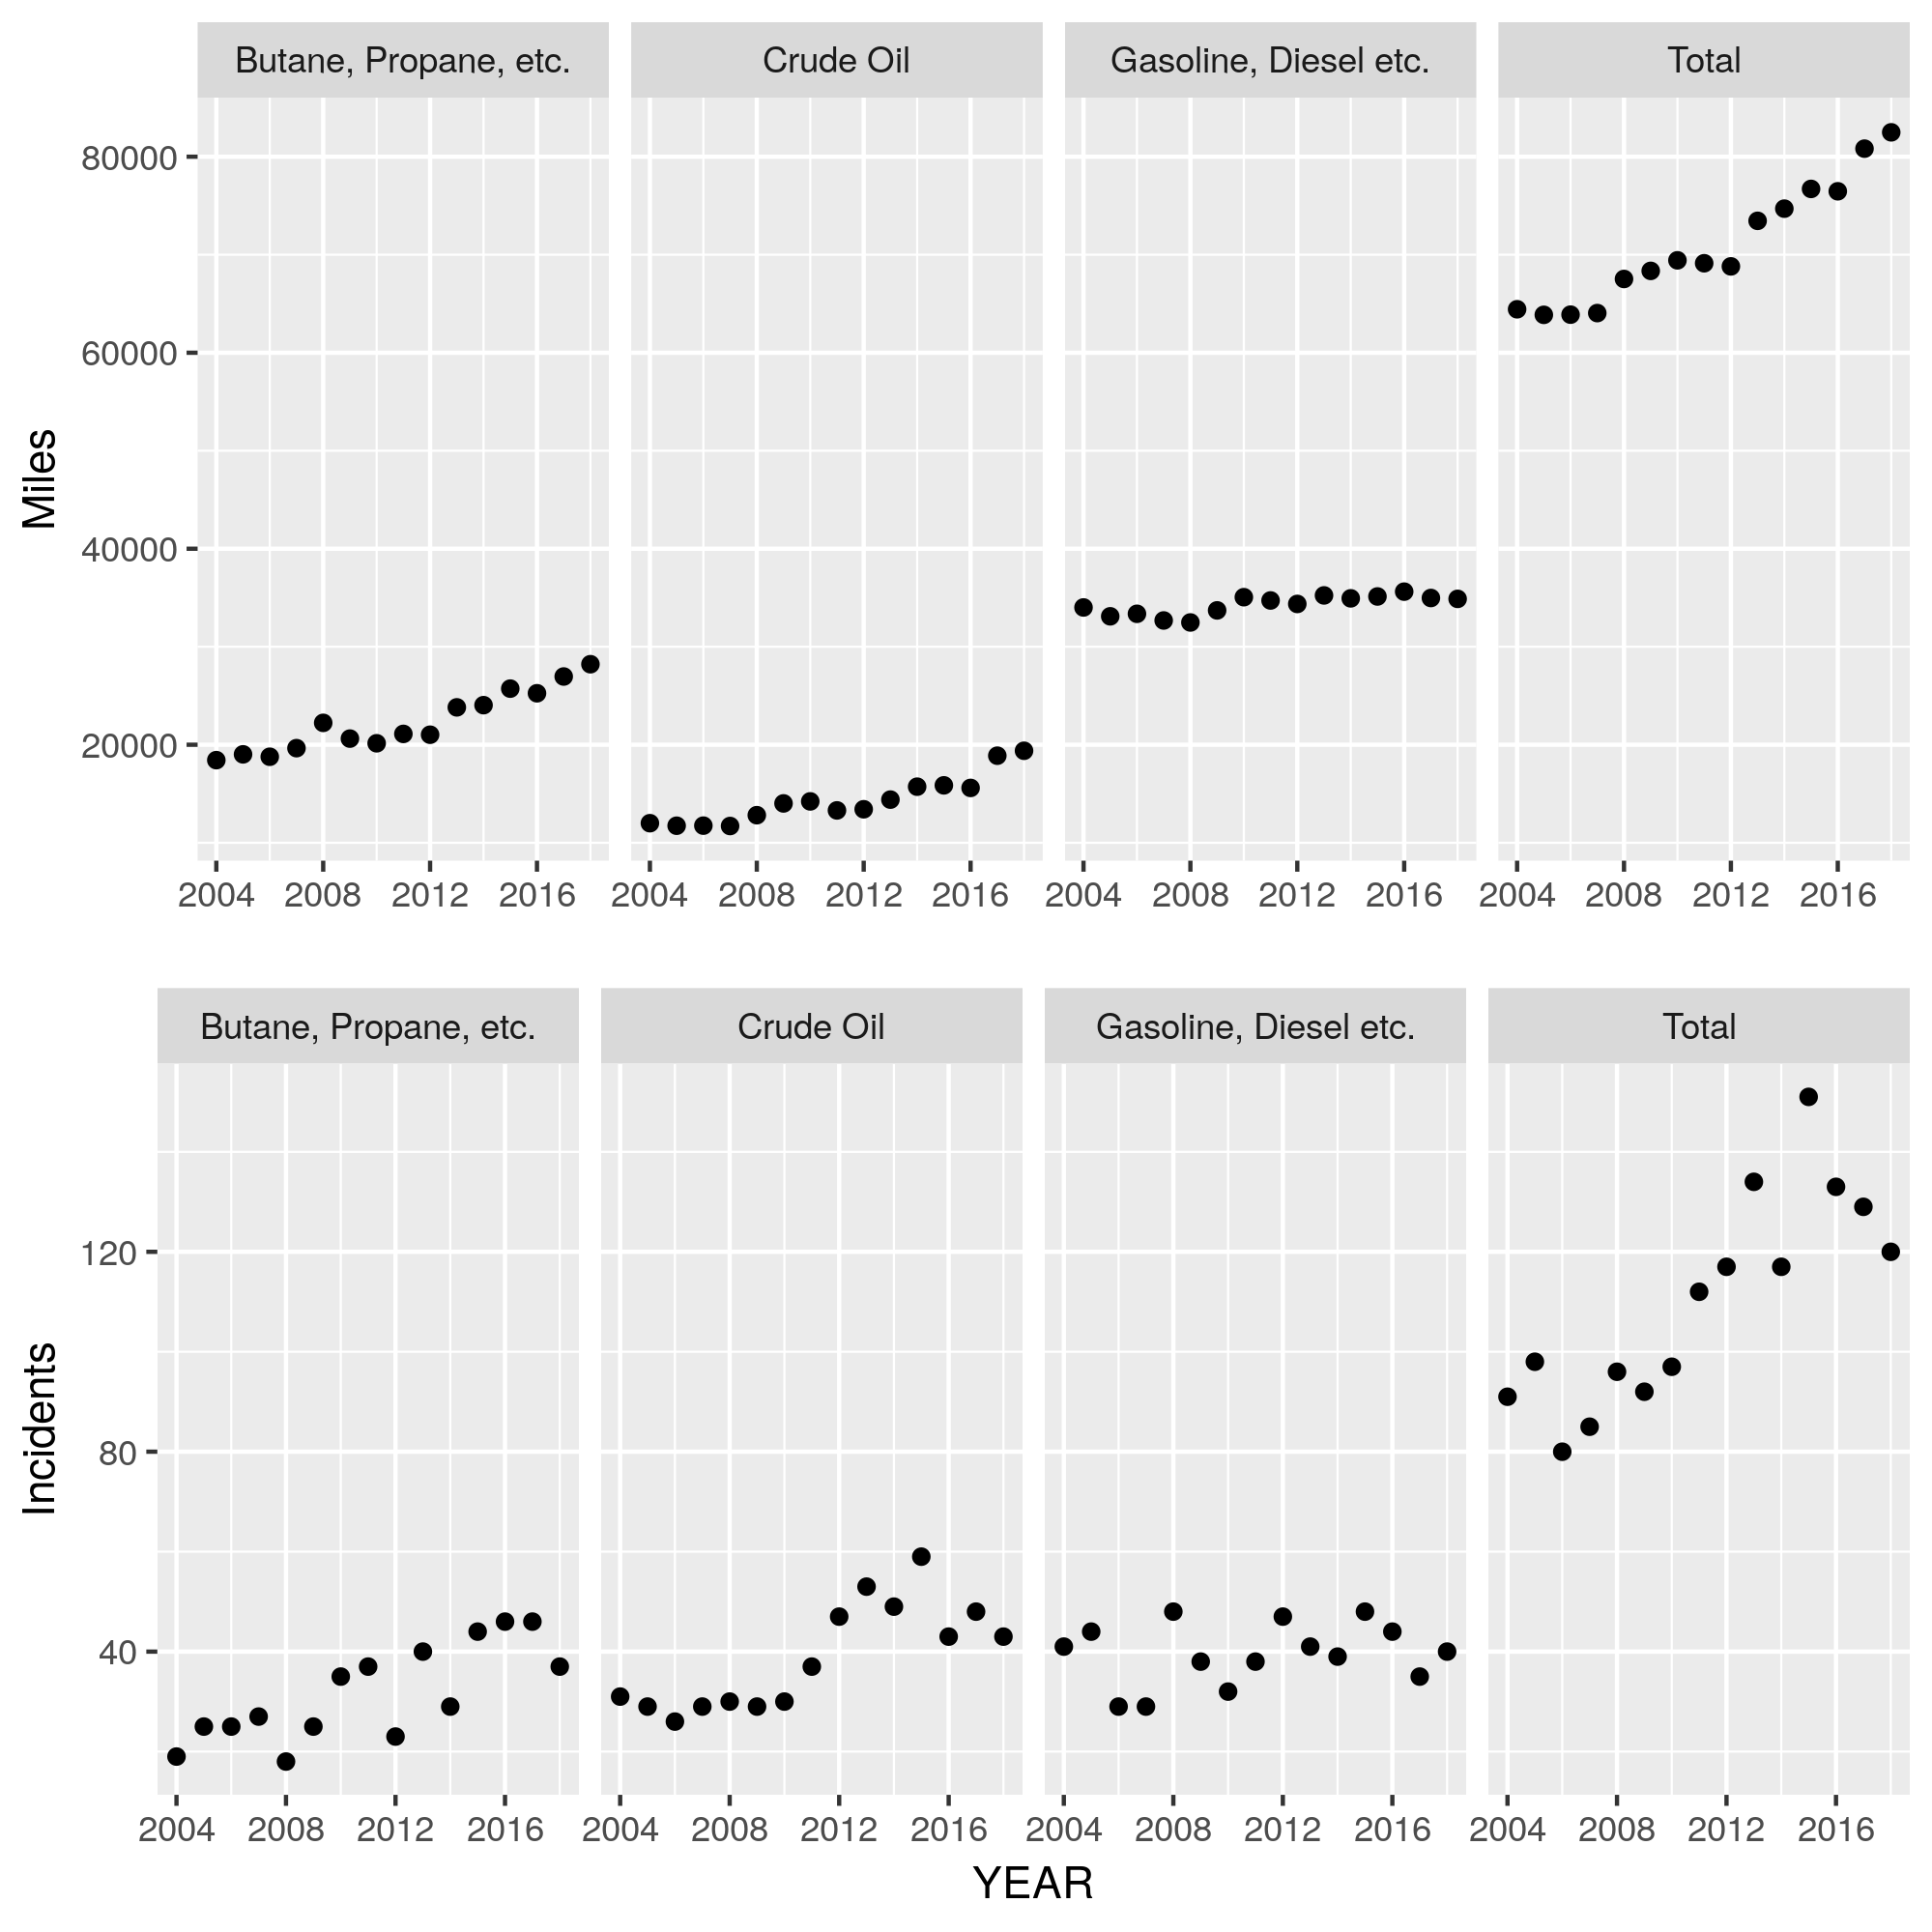
\includegraphics{illustrations/variables.png}
	\caption{}
\end{figure}

{\centering
	//////////////////////////////////////////////////////////////////////////////

	[Insert Figure 2 approximately here]

	//////////////////////////////////////////////////////////////////////////////\par
}

\begin{figure}
		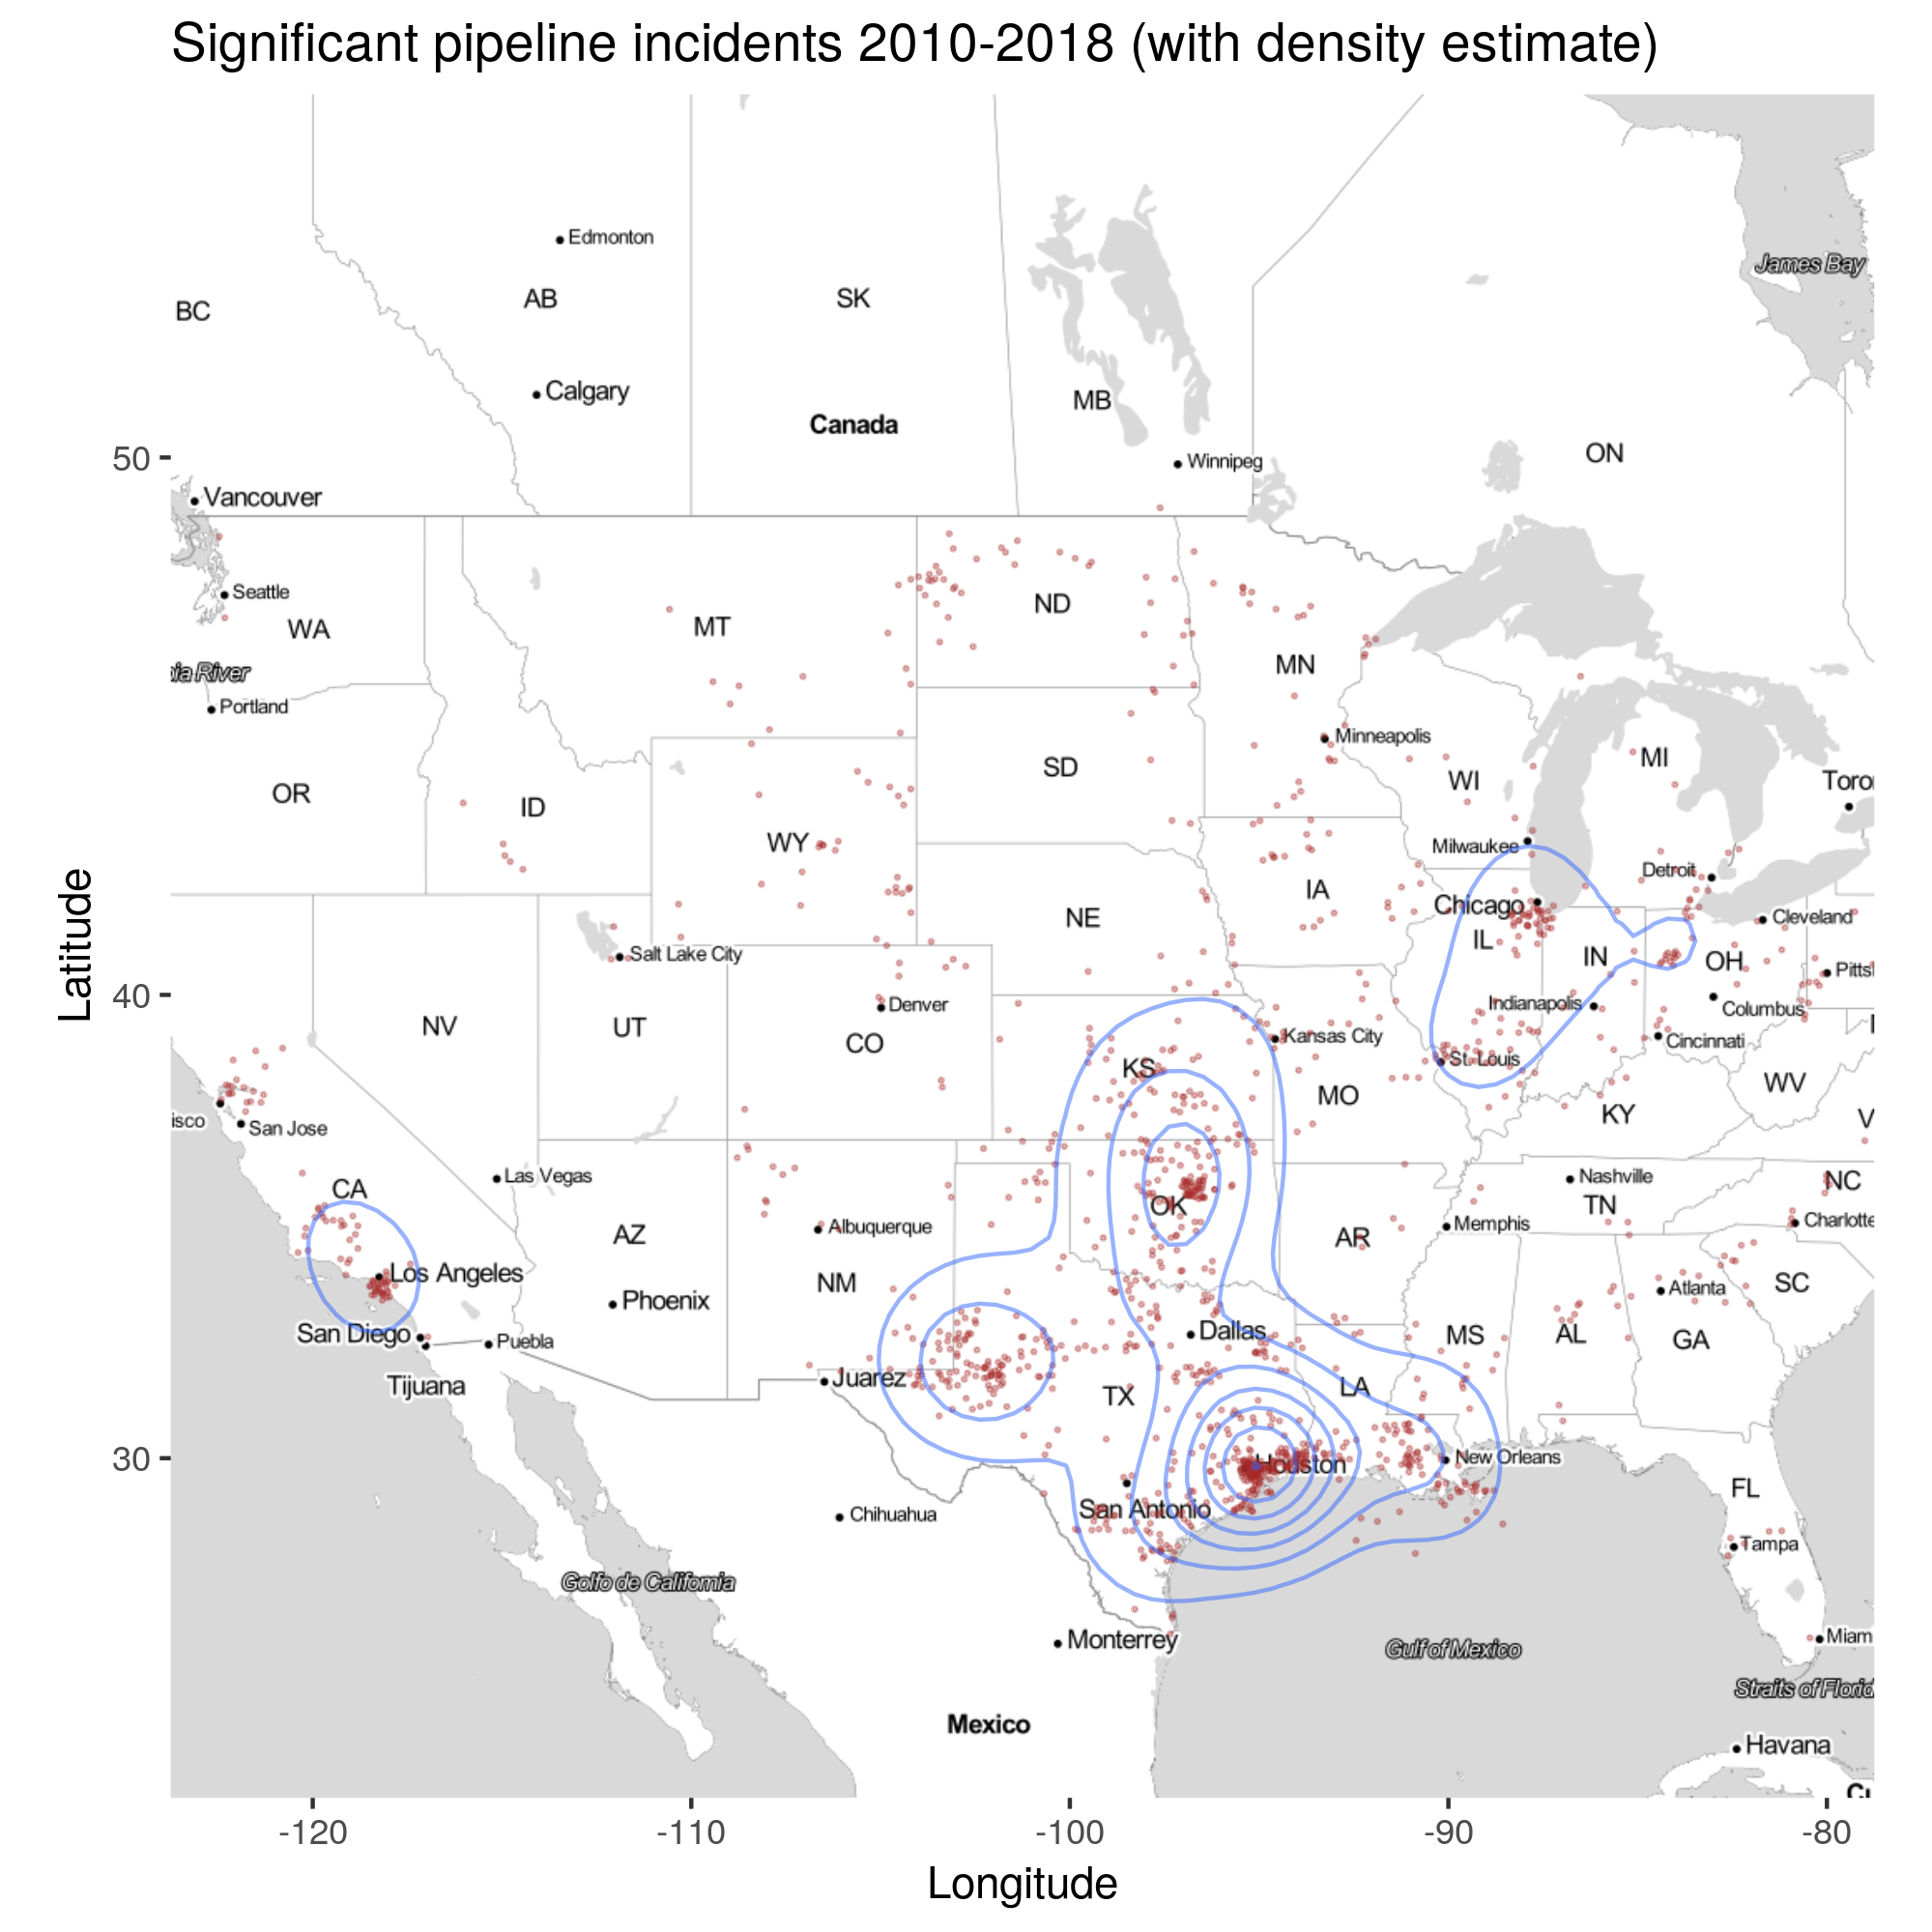
\includegraphics{illustrations/incidents.png}
		\caption{}
\end{figure}

The pipeline data has some shortcomings that we have addressed as well as possible. The data is not consolidated to the organization level. In many cases, for historic (M\&As) or legal reasons (joint ventures), even tightly controlled subsidiaries report their data separately. To address this issue, we selected the 200 largest observations in the data set (by peak pipeline miles per operator in any year of the observation period) and entered the legal names of these organizations into LexisNexis to retrieve the owners of the organziations. We also obtained from LexisNexis information on any past M\&A activities involving these organizations. We then conciliated the organizations to the group level where necessary, and used the resulting dataset for our analysis. Overall, 97 organizations belonged to 30 different company groups and we identified 7 separate M\&A events involving 6 different entities as reported by FERC, and 5 of the company groups that were identified by us. Four of the five largest operators in our sample are company groups that we have identified this way (see Figure 3). We have removed from the dataset information on CO2 pipelines (used for carbon capture and storage) and on biofuel pipelines: the definition and reporting of these pipeline types is not consistent between the reporting periods 2004-2009 and 2010-present, and the number of incidents related to these types of pipelines is low. We also did not include information on offshore pipelines in the dataset for the regression. Finally, we consolidated the incidents data to the organization level. We are controlling for the miles of pipelines for the three different commodities in the model; the residuals are the effects from organization effects that affect the pipeline network as a whole, regardless of the commodity transported: the effects of a pipeline management that successfully monitors pipelines, carries out maintenance, and reacts to stakeholder reports to prevent incidents (or fails to do any or all of that).

{\centering
	//////////////////////////////////////////////////////////////////////////////
	
	[Insert Figure 3 approximately here]
	
	//////////////////////////////////////////////////////////////////////////////\par
}

\begin{figure}
	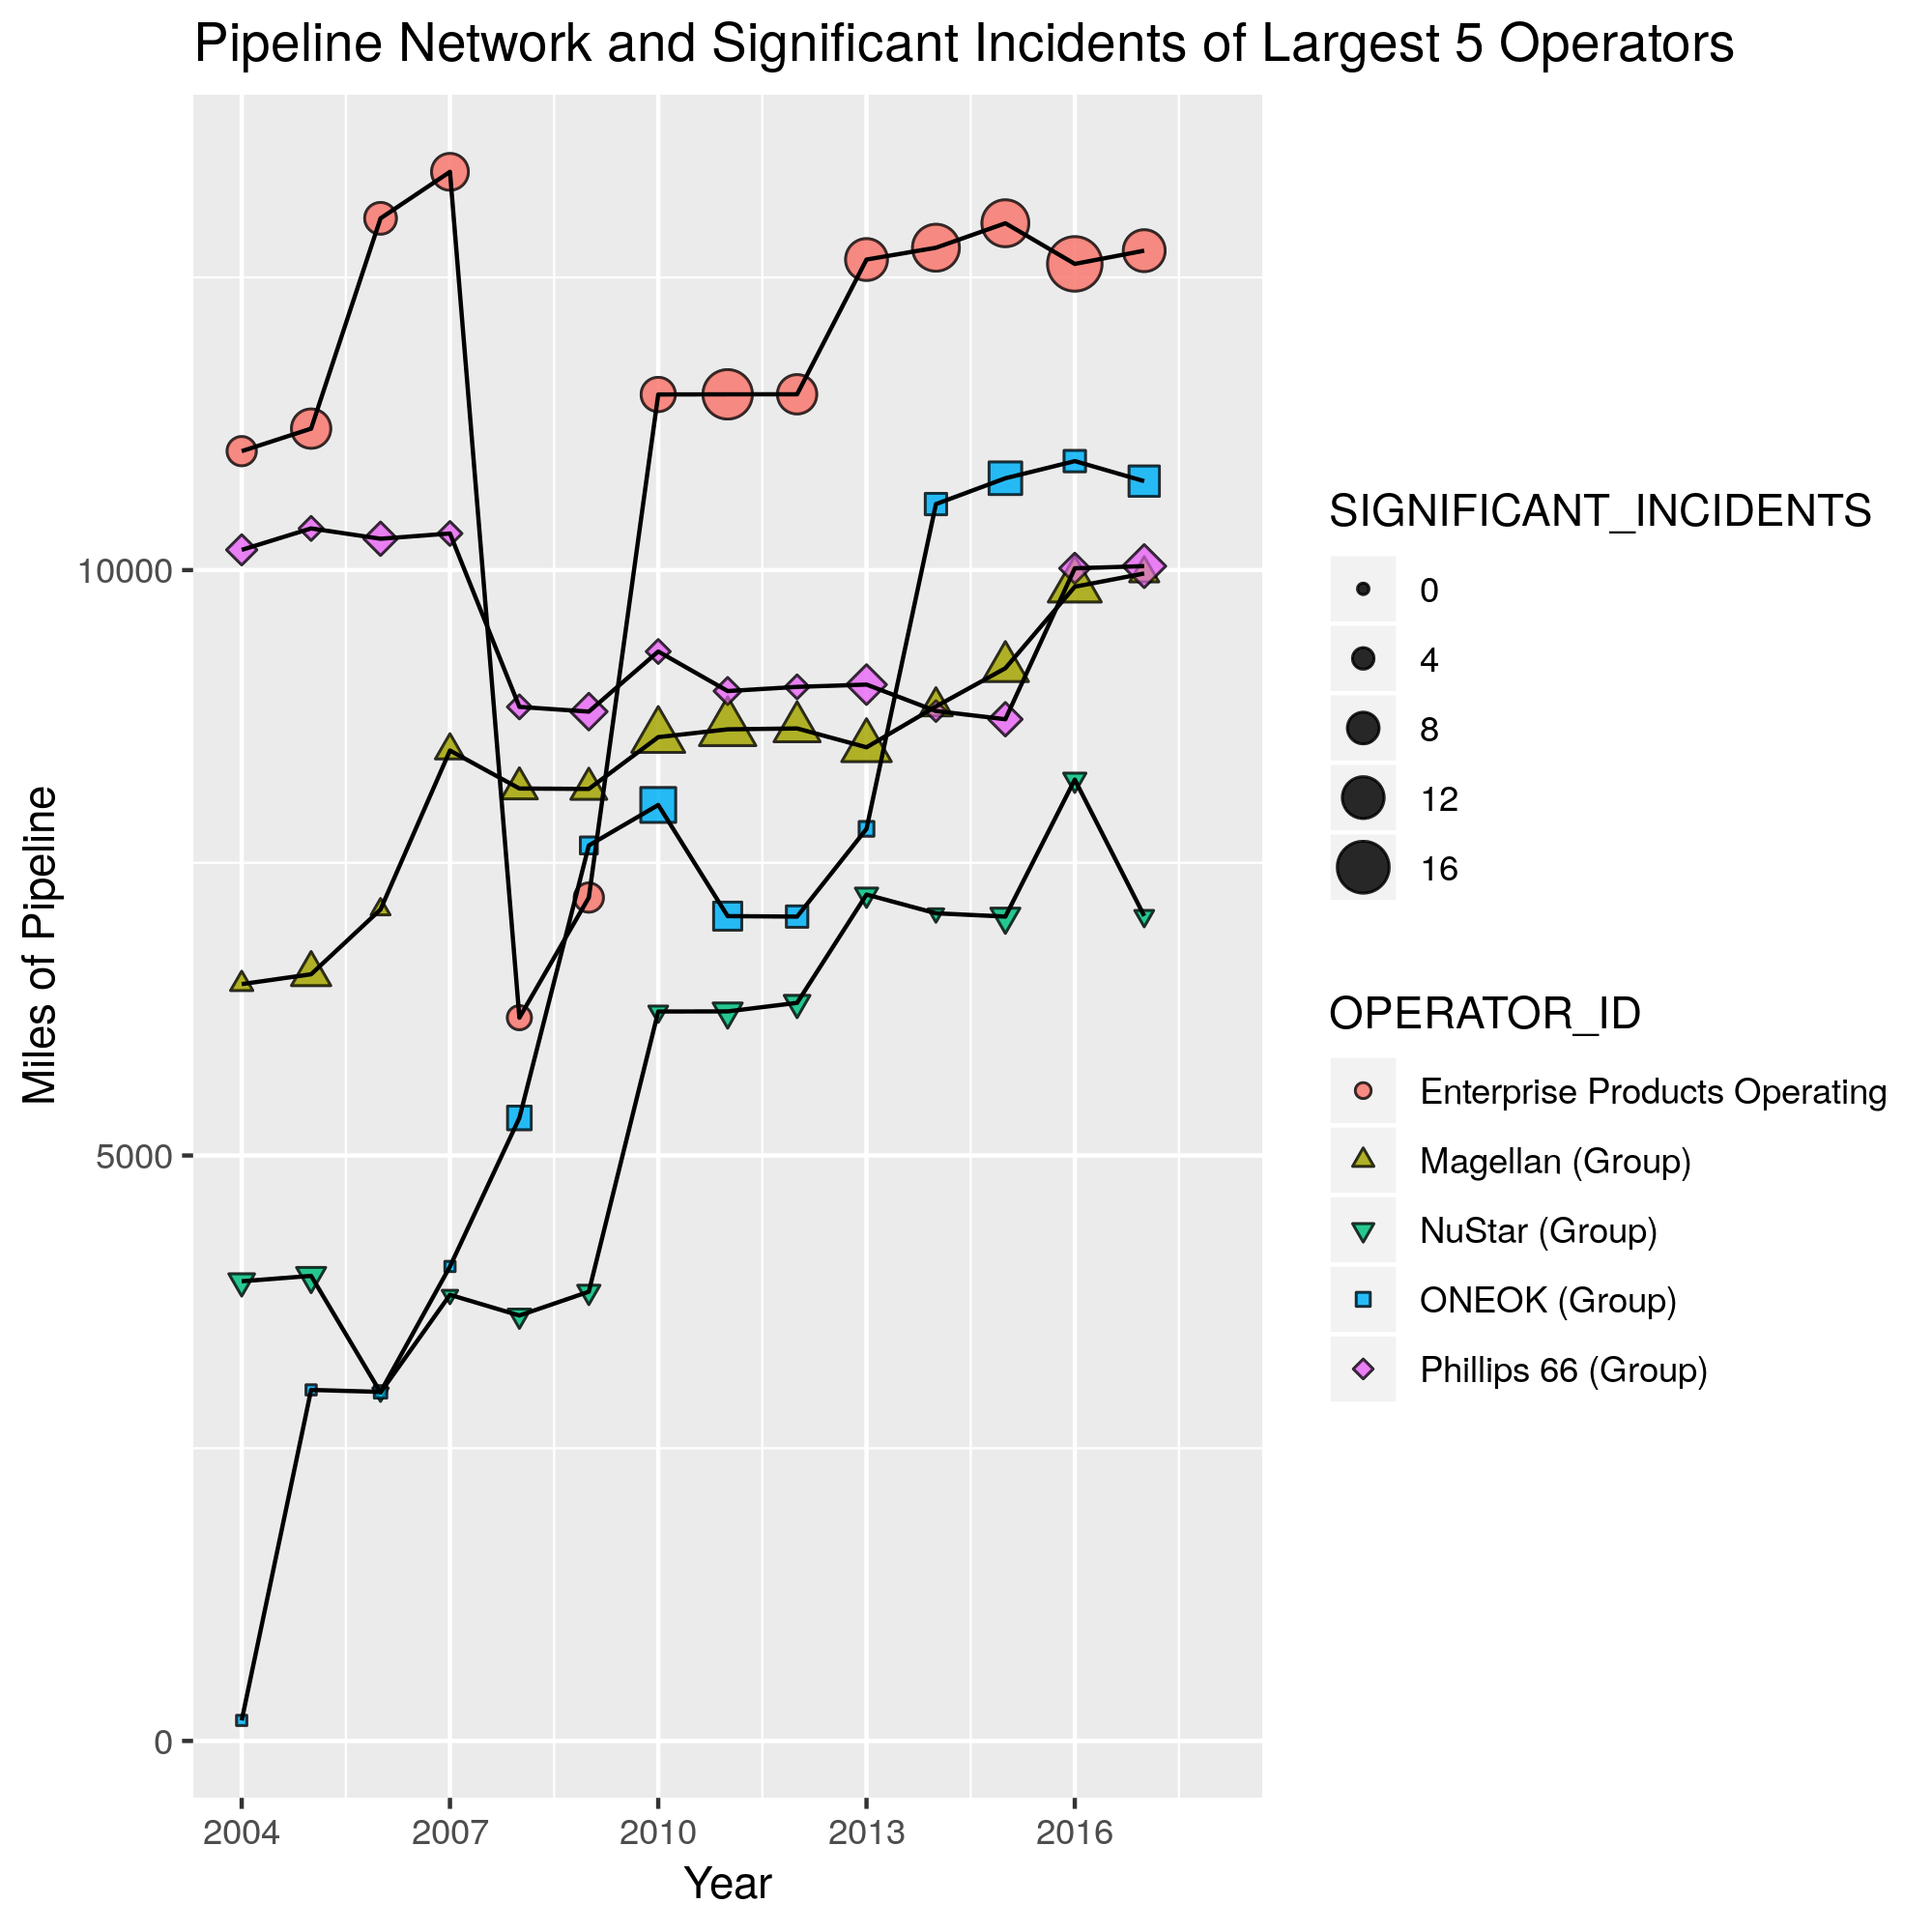
\includegraphics{illustrations/large_operators.png}
	\caption{}
\end{figure}

\subsection{Dependent variable}

We use the three-years moving average of significant pipeline incidents. A significant incident is one that either (1) caused an injury or fatality (2) \$50,000 in damage (in 1984 dollars), (3) involved the release of 5 barrels of liquid (or 50 barrels of gases such as Butane, Propane, etc.), or (4) led to an unintentional explosion or fire \citep{PHMSA}. Because the relationships described in this article play out over longer periods of time, a multi-year moving average of significant incidents ($i$) is a suitable modeling approach ($\bar{I} = (I_{t} + I_{t+1} + I_{t+2})/3$). As an added benefit, this approach further allowed us to calculate an independent variable that captures changes in strategy over a multi-year period; because the observations are only available as company-year data, we would not have been able to capture intra-year changes.

\subsection{Independent variable}

We capture both strategic adjustments, and phases of stability based on the changes that are being made to the pipeline network. To capture this, we calculate the year-over-year change $C$ (in percent) to the pipeline network $M$ ($C_{t} = M_{t} - M_{t-1}/M_{t-1}$) and then took the standard deviation of these values over a three-year period to obtain strategic adjustments $A$ ($A_{t} = ((C_{t} - \bar{C})^2 + (C_{t-1} - \bar{C})^2 + (C_{t-2} - \bar{C})^2) / 2$). In other words, a three-year period that saw no change to the extend of the pipeline network, or a steady increase, would have a very low value for strategic adjustments, whereas if an organization was to increases its pipeline network in the first year, \textit{abandons} some pipeline segments in the second year, and acquires new assets in the third year, this organization would yield a high value for strategic adjustments during that time period. Because the effect of adjustments or stability might grow exponentially the greater the change, and to test for the competing hypothesis H1c, we included a squared effect also.

\subsection{Control variables}

As mentioned above, we have to control for the miles of pipelines for each commodity to obtain accurate estimations. Every type of commodity has a slightly different base rate of incidents (see Figure 1), so we provide the average number of miles throughout the three year period that the DV is using. Further, there are multiple learning effects at play that we also want to control for. We control for technology by controlling for the age of the pipeline network. Models 1-3 use the average age of the pipeline network, as well as the interaction effect with the total miles of pipelines for each commodity. Models 4-6 provide more details to capture the effect of technology more precisely: these models use the number of miles constructed in each decade, for each commodity (e.g., in the year 2007, company x was operating y miles of crude pipeline originally constructed in the 1950, and y miles of crude pipeline constructed in the 1960, etc.). We are interested in the effect of strategic adjustments rather than the effects of consolidation. Whereas consolidation describes a company that is facing issues or attempts to raise its profitability by downsizing operations, strategic adjustment is a process of changing direction; we therefore constructed a measure for consolidation that measures the sell-off or abandonment of pipeline assets; this variable is added as an additional control variable in models 1, 3, 4, and 6. Further, we included control variables for M\&A events to control for some learning opportunities that may emerge from M\&As and improve pipeline safety. Finally, in addition to the control variable for pipeline age, we added in models 1, 3, 4, and 6 a control variable for pipelines miles added during the last four years, discounted for the current year, as well as t-2 and t-3: new technology will provide additional safety, and this effect is controlled for through the variables for pipeline network age -- but before new technology can exert this effect, the unfamiliar technology might exert a negative effect, while the staff familiarizes itself with the technology. This effect is distinct from the effect of adjustments and stability that we are interested in, and will occur regardless of whether changes are introduced gradually or abruptly. Finally, we included in models 1-3 control variables for there being no pipeline miles for a commodity, in order to control for a focus on one commodity, or a process of diversification. Finally, in models 3 and 6 we control for year effects.